\section{Arquitectura}

\begin{frame}{Diagrama de clases}
	\begin{figure}[H]
		\centering
		\begin{tikzpicture}
			\node[fill=white, inner sep=0pt] {
				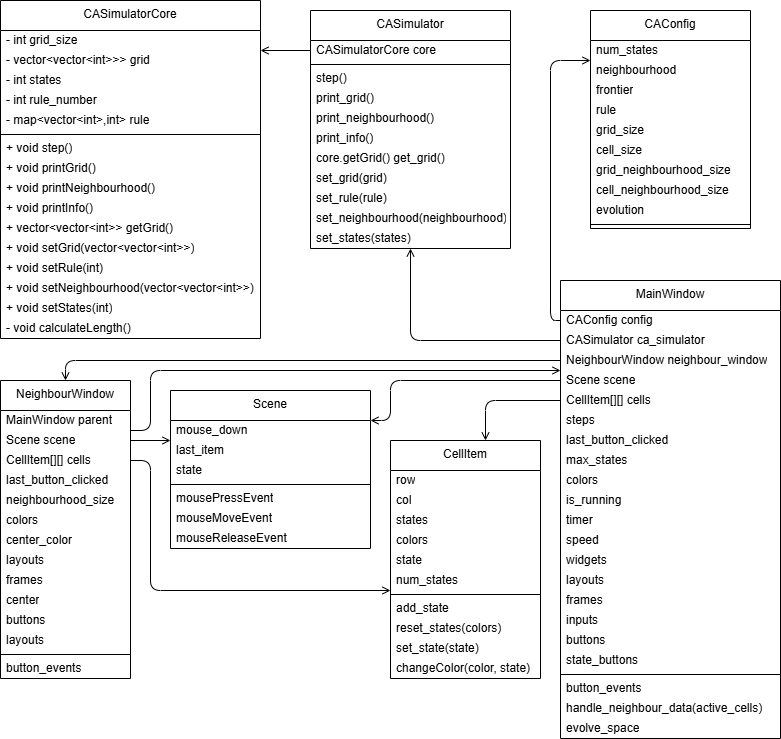
\includegraphics[width=0.5\linewidth]{images/uml_cd.png}
			};
		\end{tikzpicture}
	\end{figure}
\end{frame}


\begin{frame}{Representación del autómata celular neuronal}
	\begin{figure}[H]
		\centering
		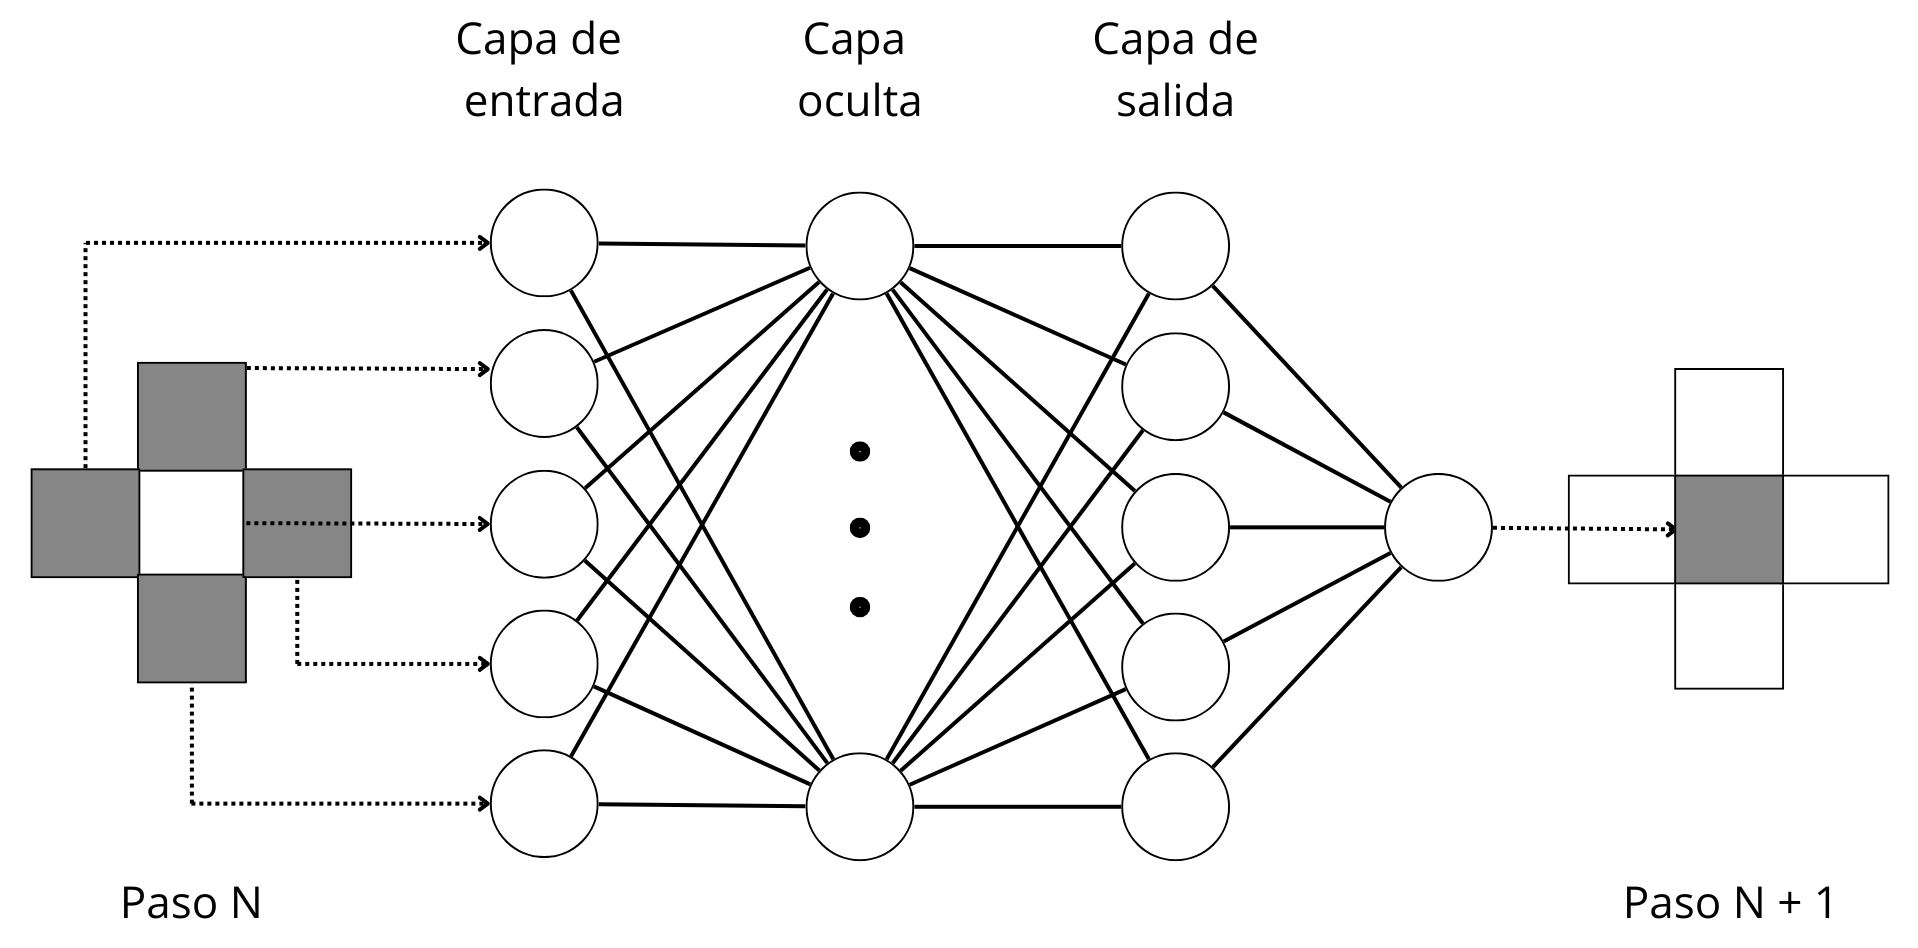
\includegraphics[width=0.6\linewidth]{images/NCA.png}
		\caption{Representación grafica de la red neuronal.}
		\label{fig:nca}
	\end{figure}
\end{frame}

\begin{frame}{Arquitectura del simulador}
	\begin{figure}[H]
		\centering
		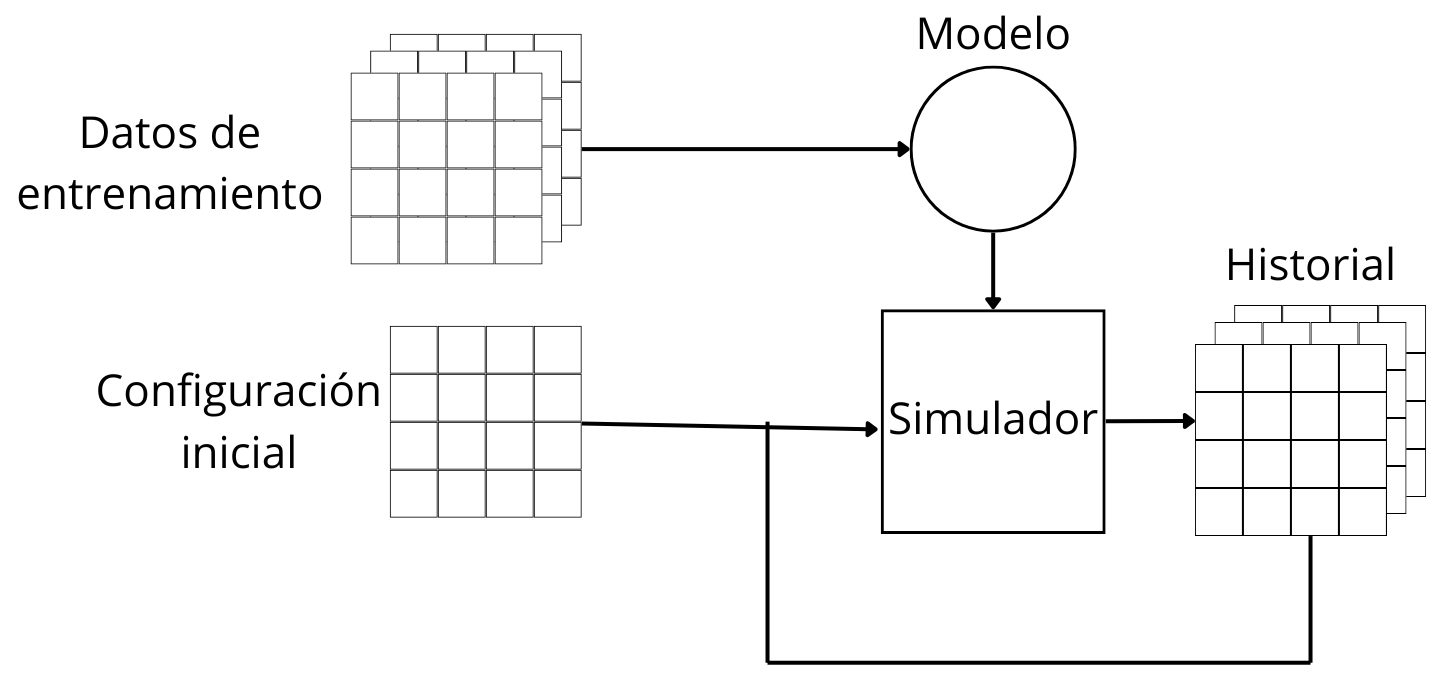
\includegraphics[width=0.6\linewidth]{images/arquitectura.png}
		\caption{Arquitectura del simulador.}
		\label{fig:arquitectura}
	\end{figure}
\end{frame}

\begin{frame}{Interfaz principal}
	\begin{figure}[H]
		\centering
		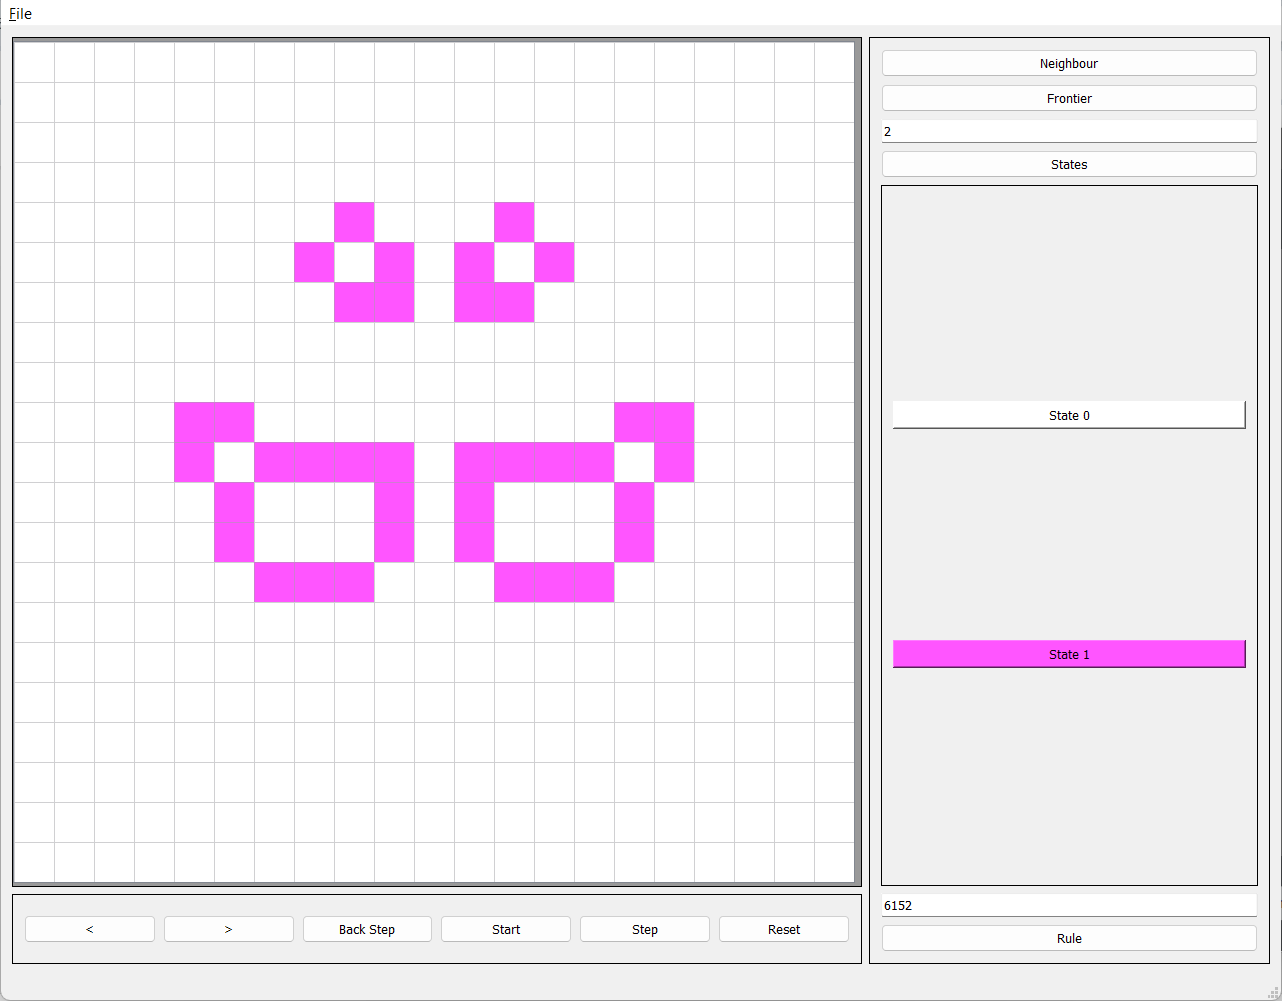
\includegraphics[width=0.45\linewidth]{images/ui_main.png}
		\caption{Interfaz principal.}
	\end{figure}
\end{frame}

\begin{frame}{Interfaz de vecindad}
	\begin{figure}[H]
		\centering
		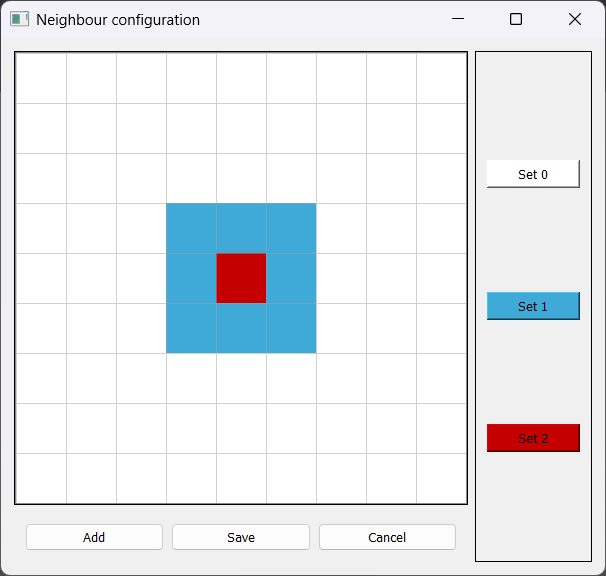
\includegraphics[width=0.45\linewidth]{images/ui_neighbour.png}
		\caption{Interfaz de vecindad.}
	\end{figure}
\end{frame}


